\subsection{\texorpdfstring{\leptonTau channel}{lepton-tau channel}}
\label{sect:leptonTauCuts}
In lepton ($e$ and $\mu$) $+$ \Tau channels, tight isolated $\Tau$ candidates with $\PT > 25 \GeV$ and $|\eta| <$ 2.3 are selected. To reduce the rate of the fake \Tau's originated from $e$ and $\mu$, the same cut as in the Higgs analysis \cite{CMS_AN_2013-171} is applied on discriminators against $e$ and $\mu$. In $e\Tau$ channel, \Tau objects which pass \emph{MediumElectronMVA3Rejection} against $e$ and the \emph{LooseMuon2Rejection} discriminator against $\mu$ are selected. In the \muTau channel, the tight working point of the \emph{Muon2Rejection} is requested and the Loose working point of the discriminator against electron is applied.

Muons with $\PT > 20 \GeVc$ and $|\eta|<2.1$ are selected in the \muTau channel. The $\mu$'s should pass tight particle flow identification and a tight cut ($<0.1$) on the isolation.
 
In $e\Tau$ channel, each event is requested to have an electron with $\PT >25 \GeVc$ in the $|\eta| < 2.1 $ region. A tight cut of $0.1$ on the isolation and $0.1$ on the $dZ$ of the selected electron are also applied.

To suppress dilepton and multilepton backgrounds, events with an extra $e$ or $\mu$ with $\PT >10 \GeV$ are rejected. In $e\Tau$ channel, for the extra electron to veto, a wider window of $|\eta|<2.3$ is scanned and a looser isolation cut of $0.2$ is applied. To find the extra $\mu$ in this channel, a selection similar to the $\mu$ selection in \muTau channel is applied. In \muTau channel, events with any extra lepton in $|\eta|<2.4$ region with isolation value $<0.3$ are vetoed. For the extra $\mu$ in this channel, no identification is requested.


After requesting two opposite sign leptons in the events, a loose cut on \MPT $(30 \GeV)$ is applied to suppress QCD events. As there is no b quark in the signal, rejecting events with one or more b-tagged jets (CSVM), with $\PT > 20 \GeV$ helps a lot in reducing \ttbar and Wb backgrounds.

To reject QCD low mass resonances, the invariant mass of the lepton and the \Tau is requested to be greater than $15\ \GeV$. Another cut on the invariant mass of the di-lepton system is applied to remove the peak of the Zjets events. It has been found that the visible mass of the $Z\to\tau\tau\to\,\ell +\Tau$ moves to $60 \pm 15 \GeV$ due to mis-reconstruction of the energy of the \Tau and also the missing energy due to the decay of the $\tau$ to electron/muom. So the events with invariant mass in the range of $[45,75]$ are cut away. The minimum angle in the transverse plane between the \MPT and the jets with \PT $>$ 40 \GeVc and $|\eta| <$ 5 is asked to be greater than 1. Figure \ref{fig:minDphi}
\begin{figure}[!Hhtb]
\centering
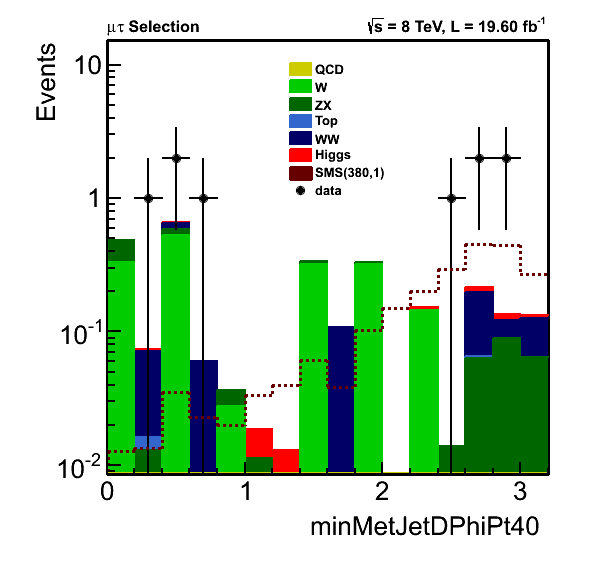
\includegraphics[angle=0,scale=0.35]{SelectionMuTau/minMetJetDPhi.png}
\caption{The minimum angle in the transverse plane between the \MPT and the jets, after all \muTau selection cuts.}
\label{fig:minDphi}
\end{figure}
shows the distribution of this variable after applying all preselection and selection cuts. This cut can kill the backgrounds, 
when the signal is almost unchanged.
As the last pre-selection cut, events with $\mttwo<40 \GeV$ are discarded to kill the bulk of the QCD events and get rid of related uncertainties due to mis-modeling and low statistics 
of the QCD events. As it has mentioned above, the signal events are expected to have high \mttwo values and are not removed with such a cut.

\begin{table}[!Hhtb]
\begin{center}
\begin{tiny}
\caption{Cut-flow-table for $e\Tau$ channel. Only statistical uncertainties are reported.}
\begin{tabular}{lccccccccc}
\hline
\hline
  & SUSY(380,1) & QCD & W & ZX & Top & WW & Higgs & MC & Data \\
\hline
\hline
\MPT,b,DiLepton Selection & 13.24&36457&26782.66&13445.54&1459.93&471.69&218.09& 78834.92$\pm$7891.60 &47988  \\
Extra Lepton Veto & 13.05&36185.38&26710.13&12689.67&1421.36&460.37&213.76& 77680.68$\pm$7886.92 &46964 \\
Z veto & 11.66&16235.65&17729.82&5170.28&1122.54&369.94&146.84& 40775.07$\pm$5220.45 &29025 \\
$\mindphifour > 1$ & 9.29&10782.87&9328.17&2900.09&545.61&179.97&90.45& 23827.15$\pm$4353.51 &16151 \\
$\mttwo > 40 \GeV$ & 6.79&140.23&3678.53&60.6&206.34&76.18&1.44& 4163.32$\pm$143.29 &4449\\
\hline
$\mttwo > 90 \GeV$ & 3.46&0.01&14.83&1.81&0.64&1.41&0.19& 18.91$\pm$4.16 &23 \\
$\tauMT > 200 \GeV$ & 2.14&0&1.29&0.38&0.02&0.05&0.06& 1.79$\pm$0.63 &3\\

\hline
\hline
\end{tabular}
\label{tbl:cutflowtableeletau}
\end{tiny}
\end{center}
\end{table}

\begin{table}[!Hhtb]
\begin{center}
\begin{tiny}
\caption{Cut-flow-table for \muTau channel. The uncertainties are just statistical.}
\begin{tabular}{lccccccccc}
\hline
\hline
  & SUSY(380,1) & QCD & W & ZX & Top & WW & Higgs & MC & Data \\
\hline
\hline
\MPT,b,DiLepton Selection  &17.03&3564.63&45555.63&28900.25&3666.78&1496.89&214.13&83398.32$\pm$2333.86 &77789\\
Extra Lepton Veto          &15.23&1966.02&44277.1&25511.77&2366.78&834.91&192.71&75149.29$\pm$1777.18 &70573\\
Z Veto                     &13.05&167.28&28857.67&5549.95&1774.94&645.79&102.55&37098.17$\pm$285.77  &35449\\
$\mindphifour > 1$         &10.75&70.56&15991.69&3540.65&912.66&351.67&75.59&20942.82$\pm$198.37  &21325\\
$\mttwo > 40 \GeV$         &7.74&0&7101.64&129.36&368.19&155.04&1.45&7755.68$\pm$122.12   &7497\\
\hline
$\mttwo > 90 \GeV$         &3.52&0&16.55&1.15&1.15&2.09&0.17&21.11$\pm$5.09       &29\\
$\tauMT > 200 \GeV$        &2.16&0&0.79&0.28&0&0.34&0.05&1.46$\pm$0.49&       5\\
%QCD 70.87 +- 34.49
%Top 1.15 +- 0.84
\hline
\hline
\end{tabular}
\label{tbl:cutflowtablemuotau}
\end{tiny}
\end{center}
\end{table}

The cut-flow-tables for the $e\Tau$ and \muTau pre-selections are shown in tables~\ref{tbl:cutflowtableeletau} and~\ref{tbl:cutflowtablemuotau} respectively. The distribution of the \PT of the \Tau and \MPT in the pre-selected events in both channels are shown in figures~\ref{fig:datamceletau} and~\ref{fig:datamcmuotau} . The good agreement between data and MC confirms that the needed correction factors are considered carefully.

\begin{figure}[!Hhtb]
\centering
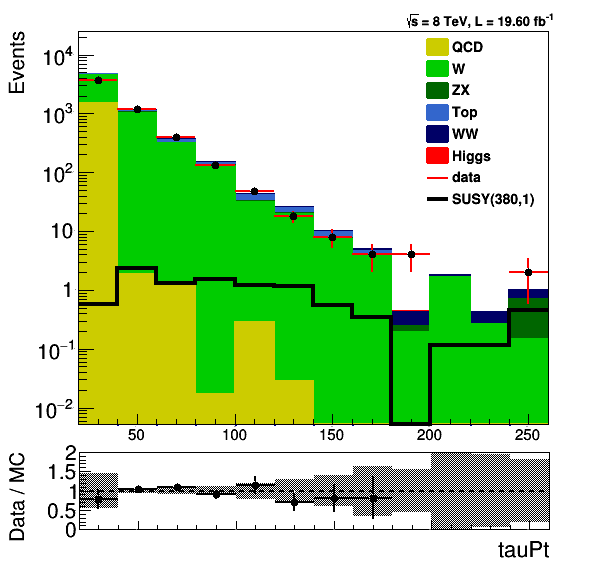
\includegraphics[angle=0,scale=0.375]{SelectionEleTau/TauPt.png}
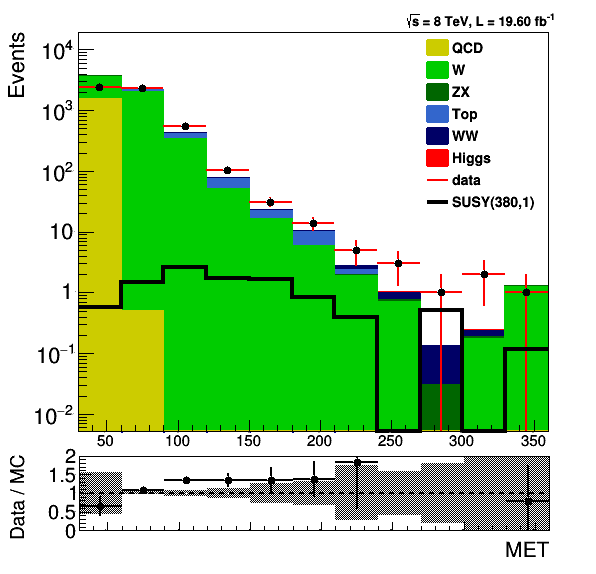
\includegraphics[angle=0,scale=0.375]{SelectionEleTau/MET.png}
\caption{Left: \Tau\PT. Right: \MPT in preselected $e\Tau$ events.}
\label{fig:datamceletau}
\end{figure}

\begin{figure}[!Hhtb]
\centering
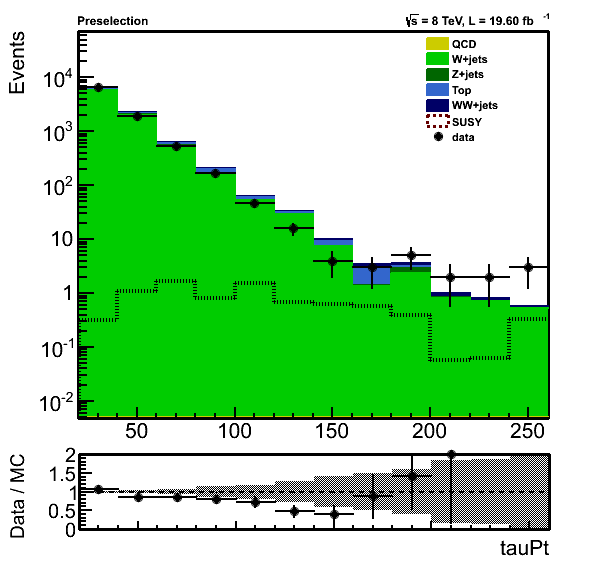
\includegraphics[angle=0,scale=0.375]{SelectionMuTau/tauPt_muTau.png}
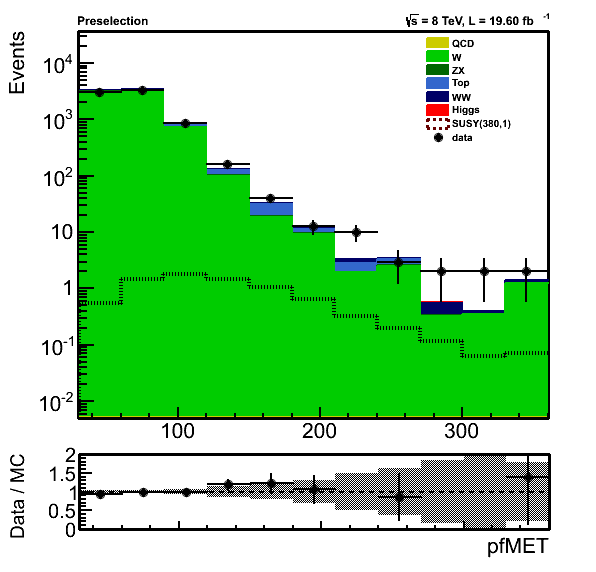
\includegraphics[angle=0,scale=0.375]{SelectionMuTau/pfMET_muTau.png}
\caption{Left: \Tau\PT. Right: \MPT in preselected \muTau events.}
\label{fig:datamcmuotau}
\end{figure}

Similar to the $\Tau\Tau$ channel, first we find the optimized cut on the \mttwo to suppress backgrounds especially \wjets events. As it has been shown in figure~\ref{fig:mt2leptontau}, the best value to cut on, similar to the $\Tau\Tau$ channel is $\mttwo > 90 \GeV$ for both $\ell\Tau$ channels. Such a high cut on the \mttwo increases the sensitivity of the study to signal events with high $\chipm$ and $\chiz$ mass differences. We then investigate the shape of different variables for signal and backgrounds and try to find the most optimized cut to have the best exclusion. The most sensitive variable for both channels are found to be the \Tau transverse mass. As it has been shown in figure~\ref{fig:taumtleptontau}, the best cut value for the high mass difference signal is $\tauMT > 200 \GeV$. The composition of the backgrounds and number of remaining signals for both channels can be found in the last row of the cut-flow-tables (tables~\ref{tbl:cutflowtableeletau} and~\ref{tbl:cutflowtablemuotau}).

\begin{figure}[!Hhtb]
\centering
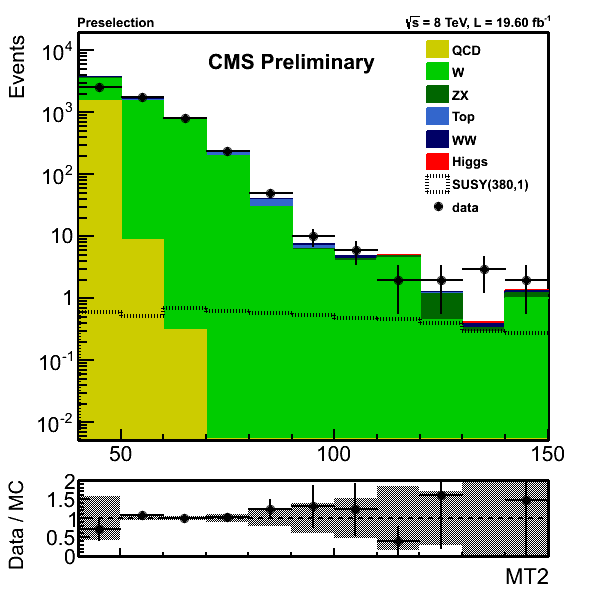
\includegraphics[angle=0,scale=0.375]{SelectionEleTau/MT2.png}
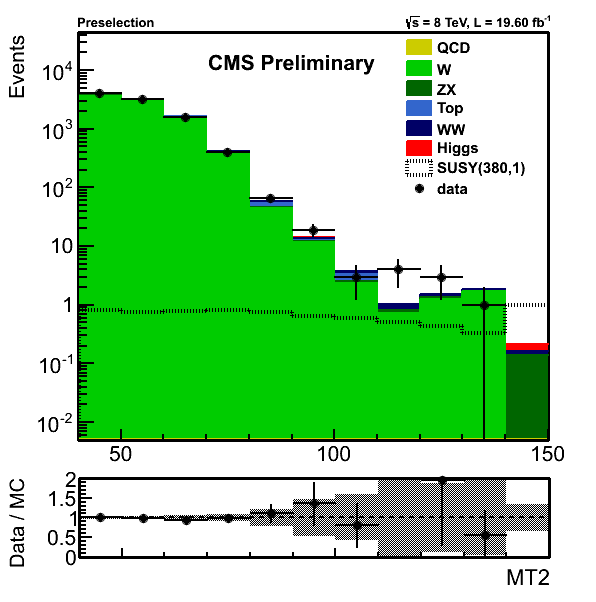
\includegraphics[angle=0,scale=0.375]{SelectionMuTau/MT2_Ratio_Preselection_unBlinded.png}
\caption{\mttwo distribution of preselected events in (Left) $e\Tau$ and (Right) \muTau channels.}
\label{fig:mt2leptontau}
\end{figure}

\begin{figure}[!Hhtb]
\centering
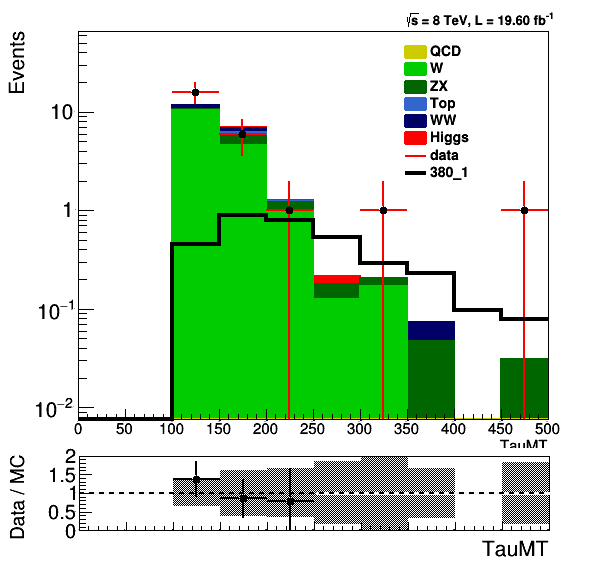
\includegraphics[angle=0,scale=0.375]{SelectionEleTau/TauMT.png}
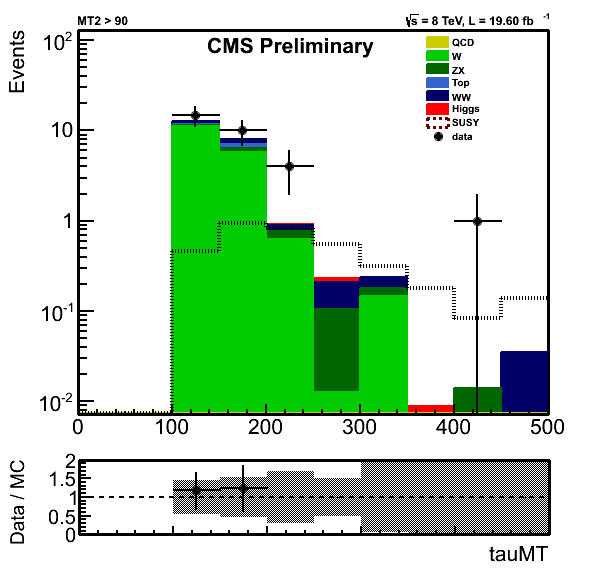
\includegraphics[angle=0,scale=0.375]{SelectionMuTau/tauMT_Ratio_MT2gt90_unBlinded.png}
\caption{\tauMT distribution for events with $\mttwo>90\GeV$ in (Left) $e\Tau$ and (Right) \muTau channels.}
\label{fig:taumtleptontau}
\end{figure}
Opposite to the \tauTau channel, the events with $\mttwo<90 \GeV$ are not useful in \leptonTau channels because of the contamination of 
the \wjets events. It was investigated if increasing the \pt of the objects can increase the sensitivity in this bin, but no improvement was seen.
The main reason can be due to the softer leptons (e and $\mu$) in the signal which come from the decay of the $\tau$'s 
to leptons plus two neutrinos ($\tau\rightarrow\ell\nu_{\ell}\nu$), 
comparing to the $W$jets backgrounds where the leptons are prompt coming from the decay of $W$ bosons.
